\documentclass[11pt,letterpaper]{article}
\usepackage[spanish]{babel}
\usepackage[T1]{fontenc}
\usepackage[utf8]{inputenc}
\usepackage{geometry}
\geometry{margin=2cm}
\usepackage{amsmath}
\usepackage{graphicx}
\usepackage{float}
\usepackage{booktabs}
\usepackage{xcolor}
\usepackage{fancyhdr}
\setlength{\headheight}{14.5pt}
\addtolength{\topmargin}{-2.5pt}
\usepackage{hyperref}
\hypersetup{colorlinks=true,linkcolor=blue,urlcolor=blue}
\usepackage{parskip}

\pagestyle{fancy}
\fancyhf{}
\rhead{Lab 12 — Evidencia Experimental}
\lhead{CC3069 Computación Paralela y Distribuida}
\cfoot{Página \thepage}

\title{\textbf{Evidencia de Ejecución y Resultados Experimentales}\\
       \large Laboratorio 12 — Speedup y Eficiencia\\
       \normalsize Computación Paralela y Distribuida (CC3069)}
\author{Javier Eduardo España Pacheco}
\date{Octubre 2026}

\begin{document}
\maketitle
\thispagestyle{fancy}

\begin{abstract}
Este documento contiene la evidencia visual de respaldo para el Laboratorio 12: capturas de la configuración del procesador (\texttt{lscpu}), la compilación exitosa del ejecutable (\texttt{make}), la ejecución completa de cada uno de los cuatro modos (\texttt{amdahl}, \texttt{suma}, \texttt{desbalance}, \texttt{gustafson}), las 7 gráficas de análisis generadas por \texttt{graficar.py}, y las pruebas del reto opcional de speedup superlineal.
\end{abstract}

\vspace{0.5cm}

\section{Datos del Equipo (lscpu)}
\begin{figure}[H]
\centering
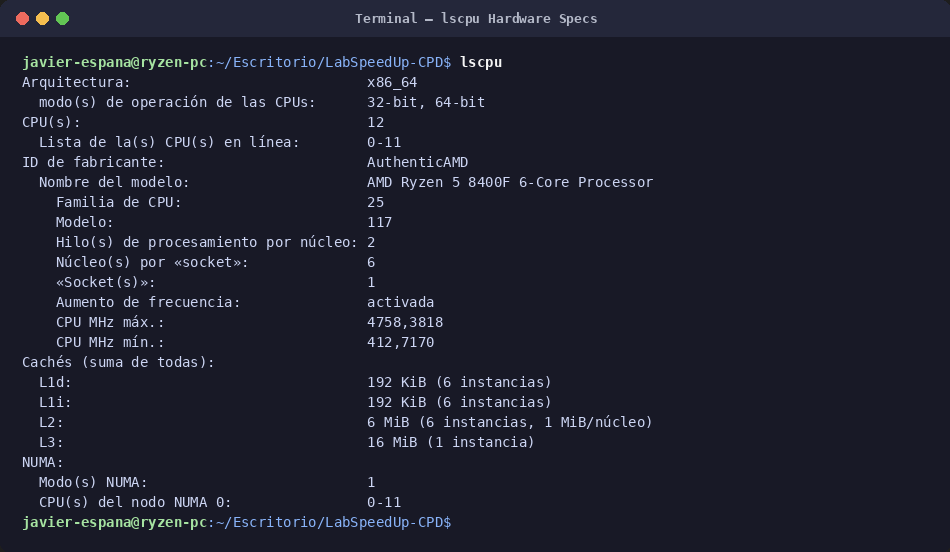
\includegraphics[width=0.95\textwidth]{captura_lscpu.png}
\caption{Captura de salida de \texttt{lscpu}: AMD Ryzen 5 8400F, 6 núcleos físicos, 12 hilos lógicos SMT, L2 de 1 MiB/núcleo y L3 compartida de 16 MiB.}
\end{figure}

\newpage
\section{Compilación y Ayuda del Programa}
\begin{figure}[H]
\centering
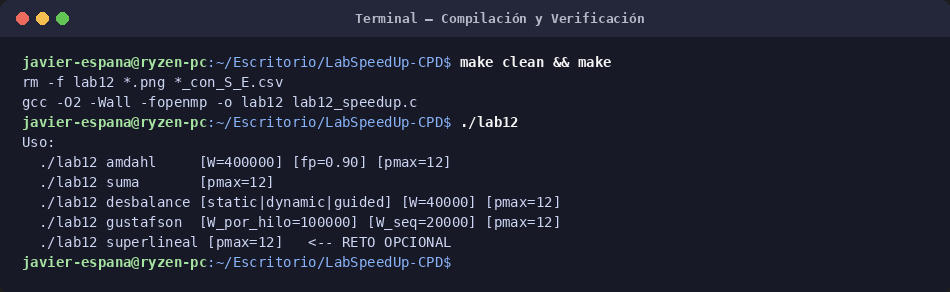
\includegraphics[width=0.95\textwidth]{captura_make.png}
\caption{Captura de compilación con \texttt{make} (GCC con \texttt{-O2 -Wall -fopenmp}) e invocación del binario mostrando su interfaz de uso.}
\end{figure}

\vspace{0.5cm}

\section{Ejecución de los 4 Modos Experimentales}

\subsection{Modo 1: Ley de Amdahl (Problema Fijo)}
\begin{figure}[H]
\centering
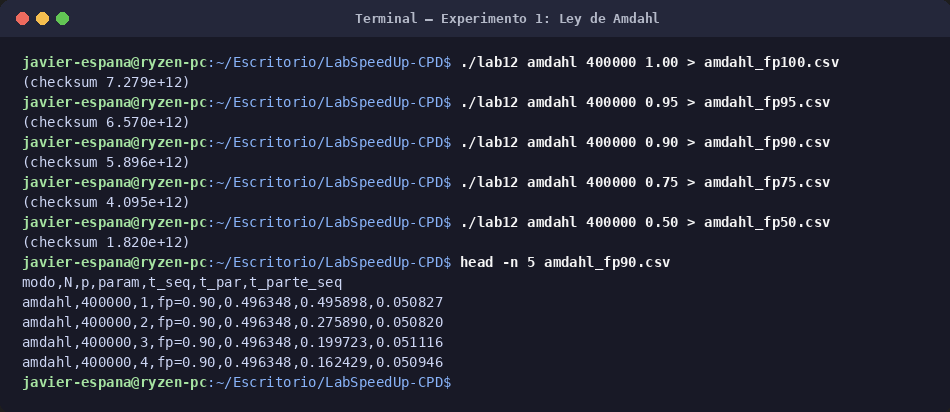
\includegraphics[width=0.95\textwidth]{captura_amdahl.png}
\caption{Ejecución del modo \texttt{amdahl} para los 5 valores de fracción paralelizable $f_p \in \{1.00, 0.95, 0.90, 0.75, 0.50\}$.}
\end{figure}

\newpage
\subsection{Modo 2: Granularidad (Suma de $N$ Números)}
\begin{figure}[H]
\centering
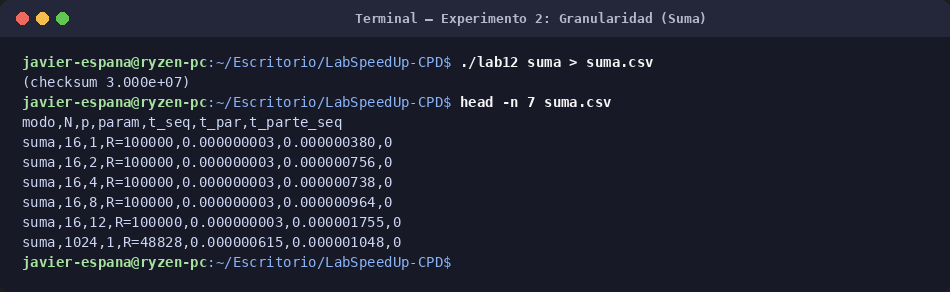
\includegraphics[width=0.95\textwidth]{captura_suma.png}
\caption{Ejecución del modo \texttt{suma} para tamaños desde $N=16$ hasta $N=16{,}777{,}216$ elementos.}
\end{figure}

\vspace{0.5cm}

\subsection{Modo 3: Desbalance de Carga (Scheduling)}
\begin{figure}[H]
\centering
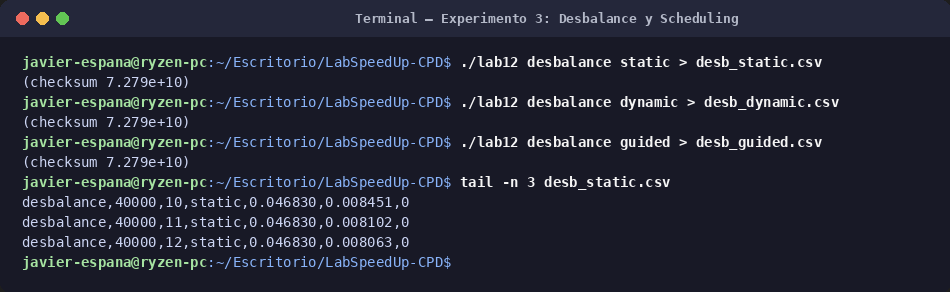
\includegraphics[width=0.95\textwidth]{captura_desbalance.png}
\caption{Ejecución del modo \texttt{desbalance} evaluando las tres políticas: \texttt{static}, \texttt{dynamic} y \texttt{guided}.}
\end{figure}

\newpage
\subsection{Modo 4: Ley de Gustafson (Problema Creciente)}
\begin{figure}[H]
\centering
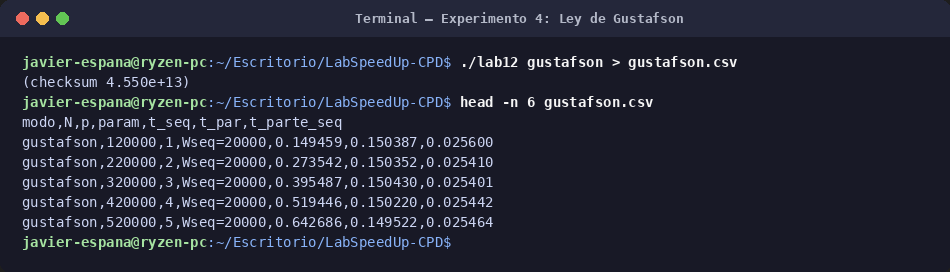
\includegraphics[width=0.95\textwidth]{captura_gustafson.png}
\caption{Ejecución del modo \texttt{gustafson} con trabajo por hilo fijo ($W_{\text{hilo}} = 100{,}000$) y parte secuencial fija ($W_{\text{seq}} = 20{,}000$).}
\end{figure}

\vspace{0.5cm}

\subsection{Reto Opcional: Speedup Superlineal}
\begin{figure}[H]
\centering
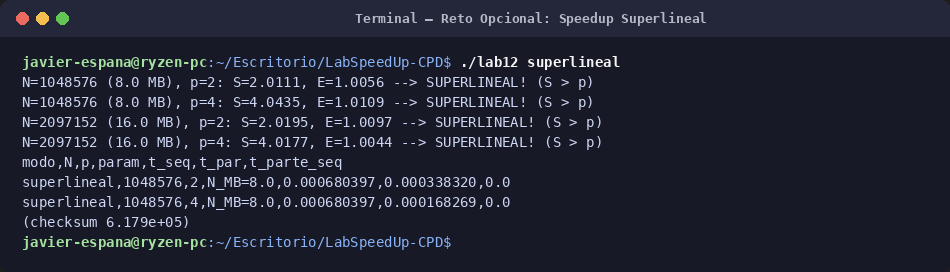
\includegraphics[width=0.95\textwidth]{captura_superlineal.png}
\caption{Ejecución del modo \texttt{superlineal} demostrando $S > p$ repetible debido al ajuste en jerarquía de caché L2/L3.}
\end{figure}

\newpage
\section{Las 7 Gráficas Generadas por \texttt{graficar.py}}

\subsection{Parte 1: Amdahl (Gráficas 1 y 2)}
\begin{figure}[H]
\centering
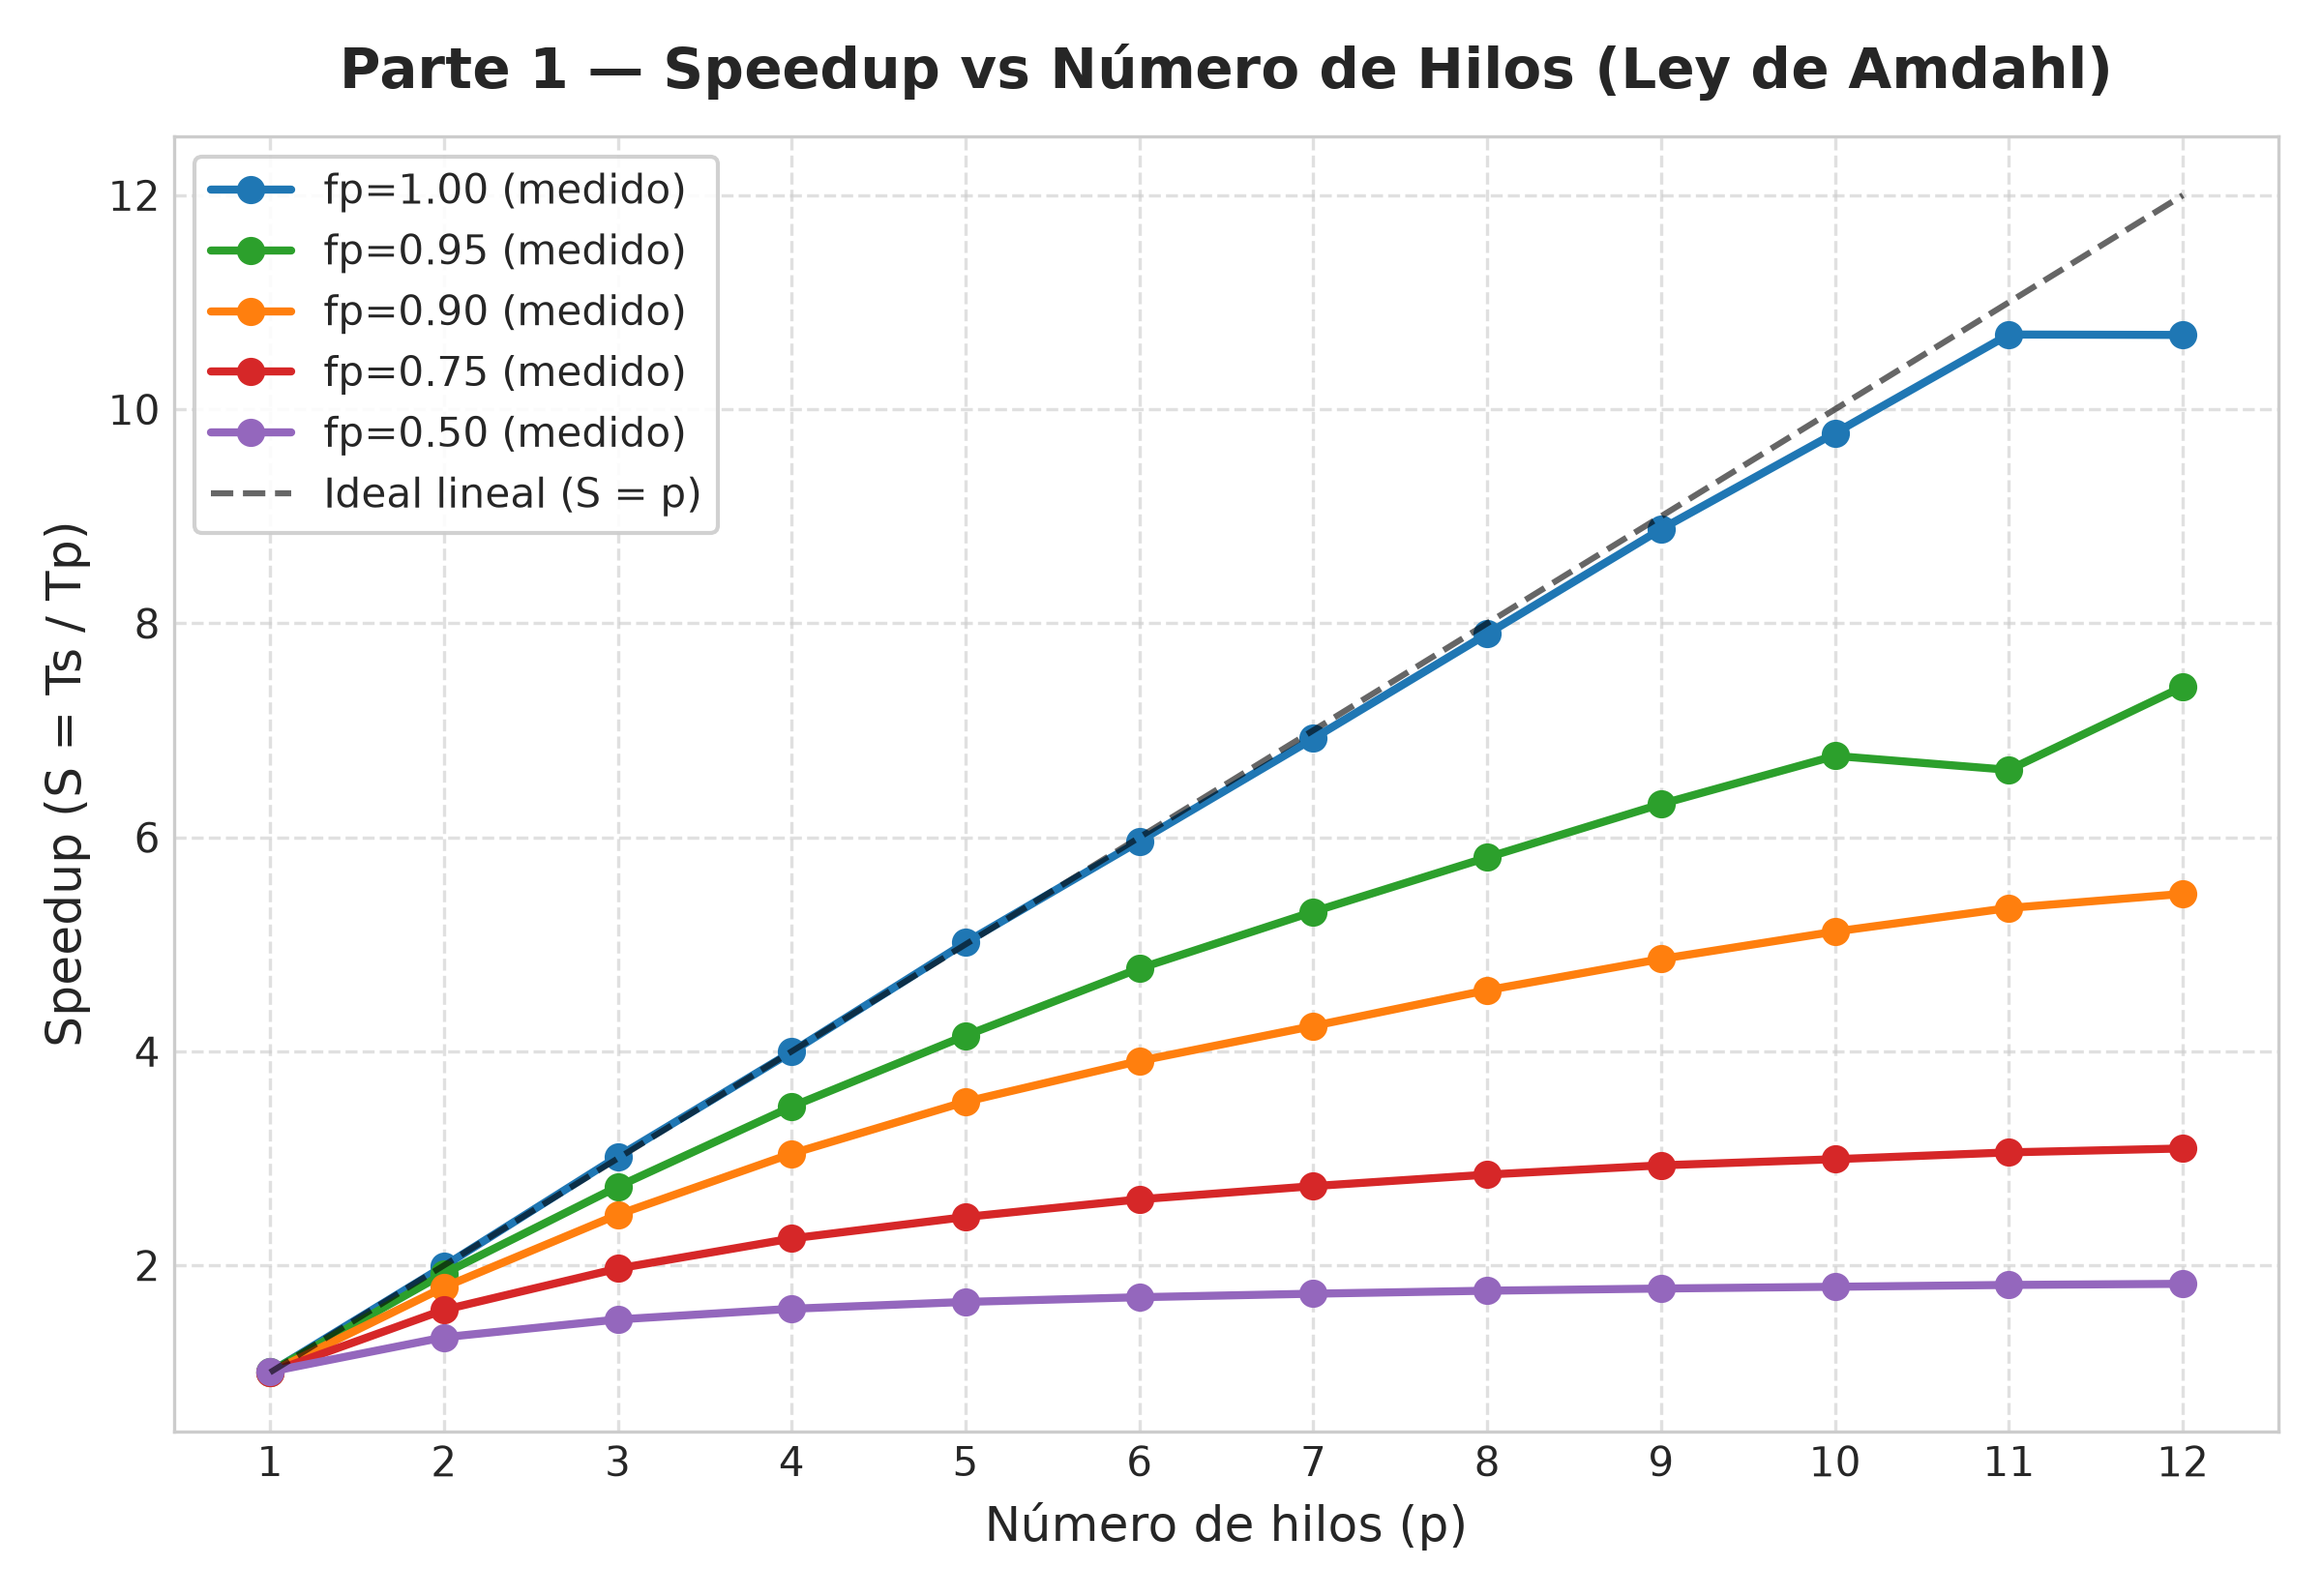
\includegraphics[width=0.88\textwidth]{grafica_amdahl_speedup.png}
\caption{Gráfica 1 — Speedup $S$ vs. hilos ($p$) para cada fracción paralelizable $f_p$.}
\end{figure}

\begin{figure}[H]
\centering
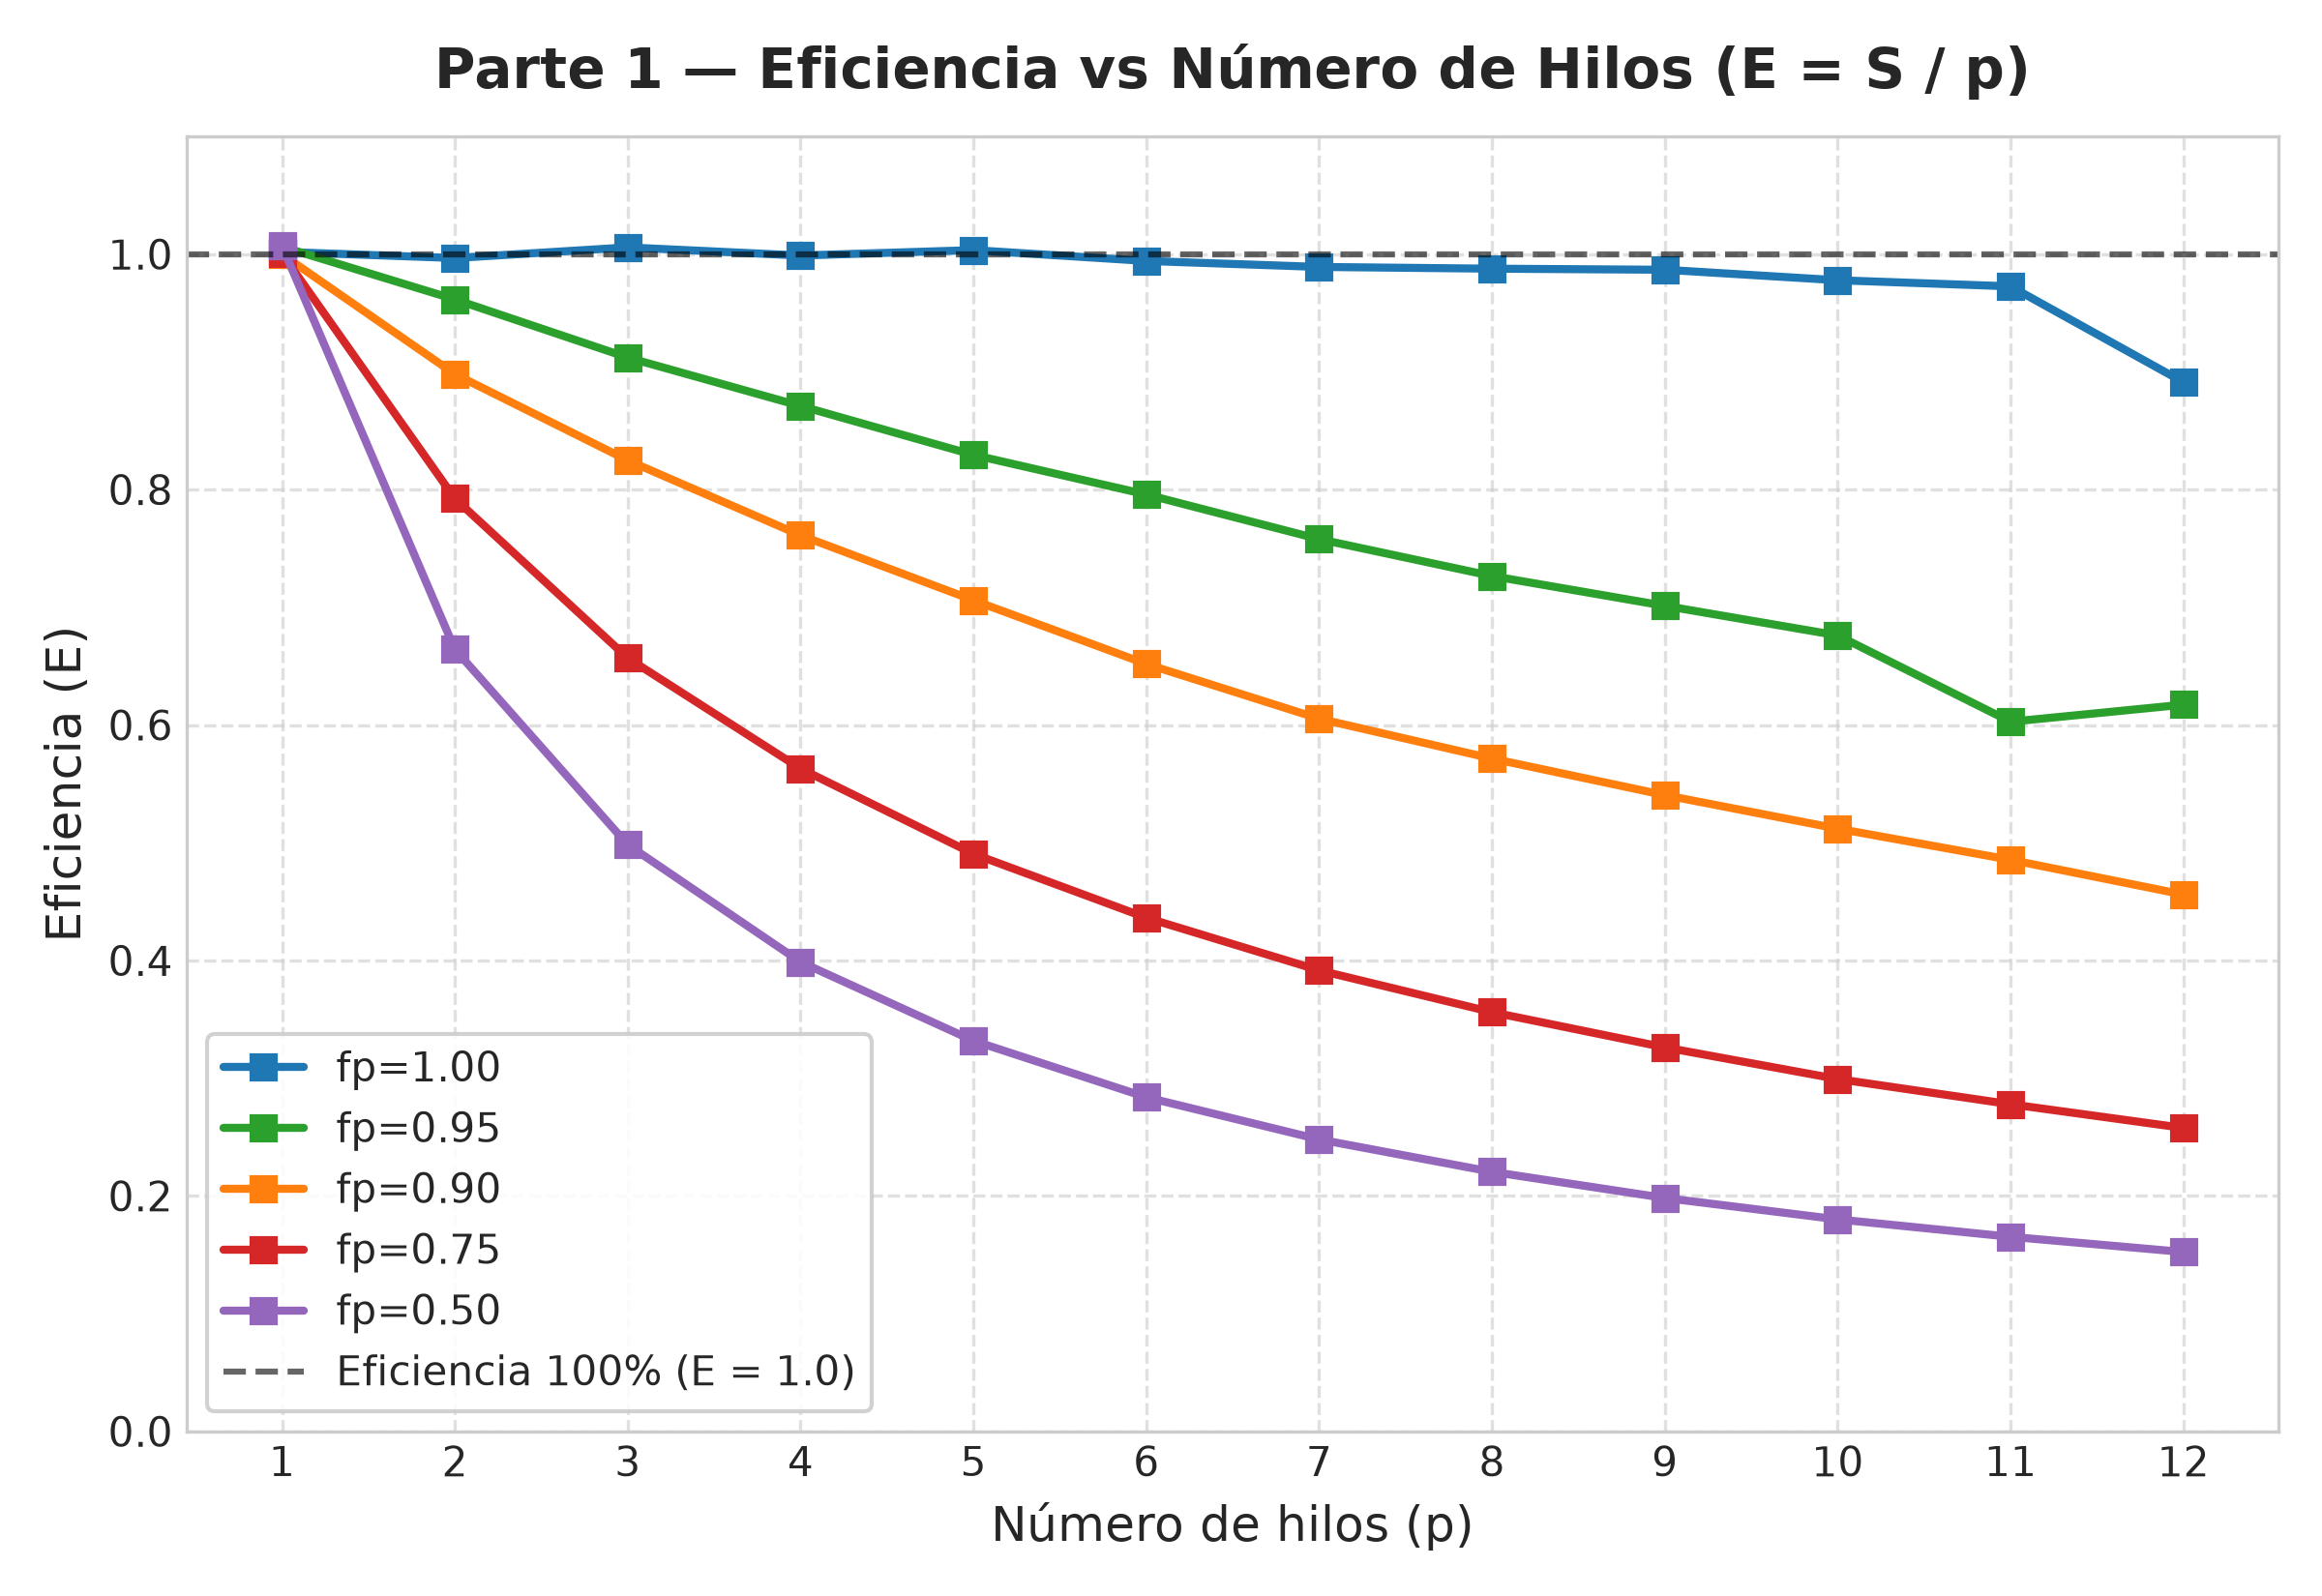
\includegraphics[width=0.88\textwidth]{grafica_amdahl_eficiencia.png}
\caption{Gráfica 2 — Eficiencia $E = S/p$ vs. hilos ($p$) para cada fracción paralelizable.}
\end{figure}

\newpage
\subsection{Parte 2: Granularidad en Suma (Gráficas 3 y 4)}
\begin{figure}[H]
\centering
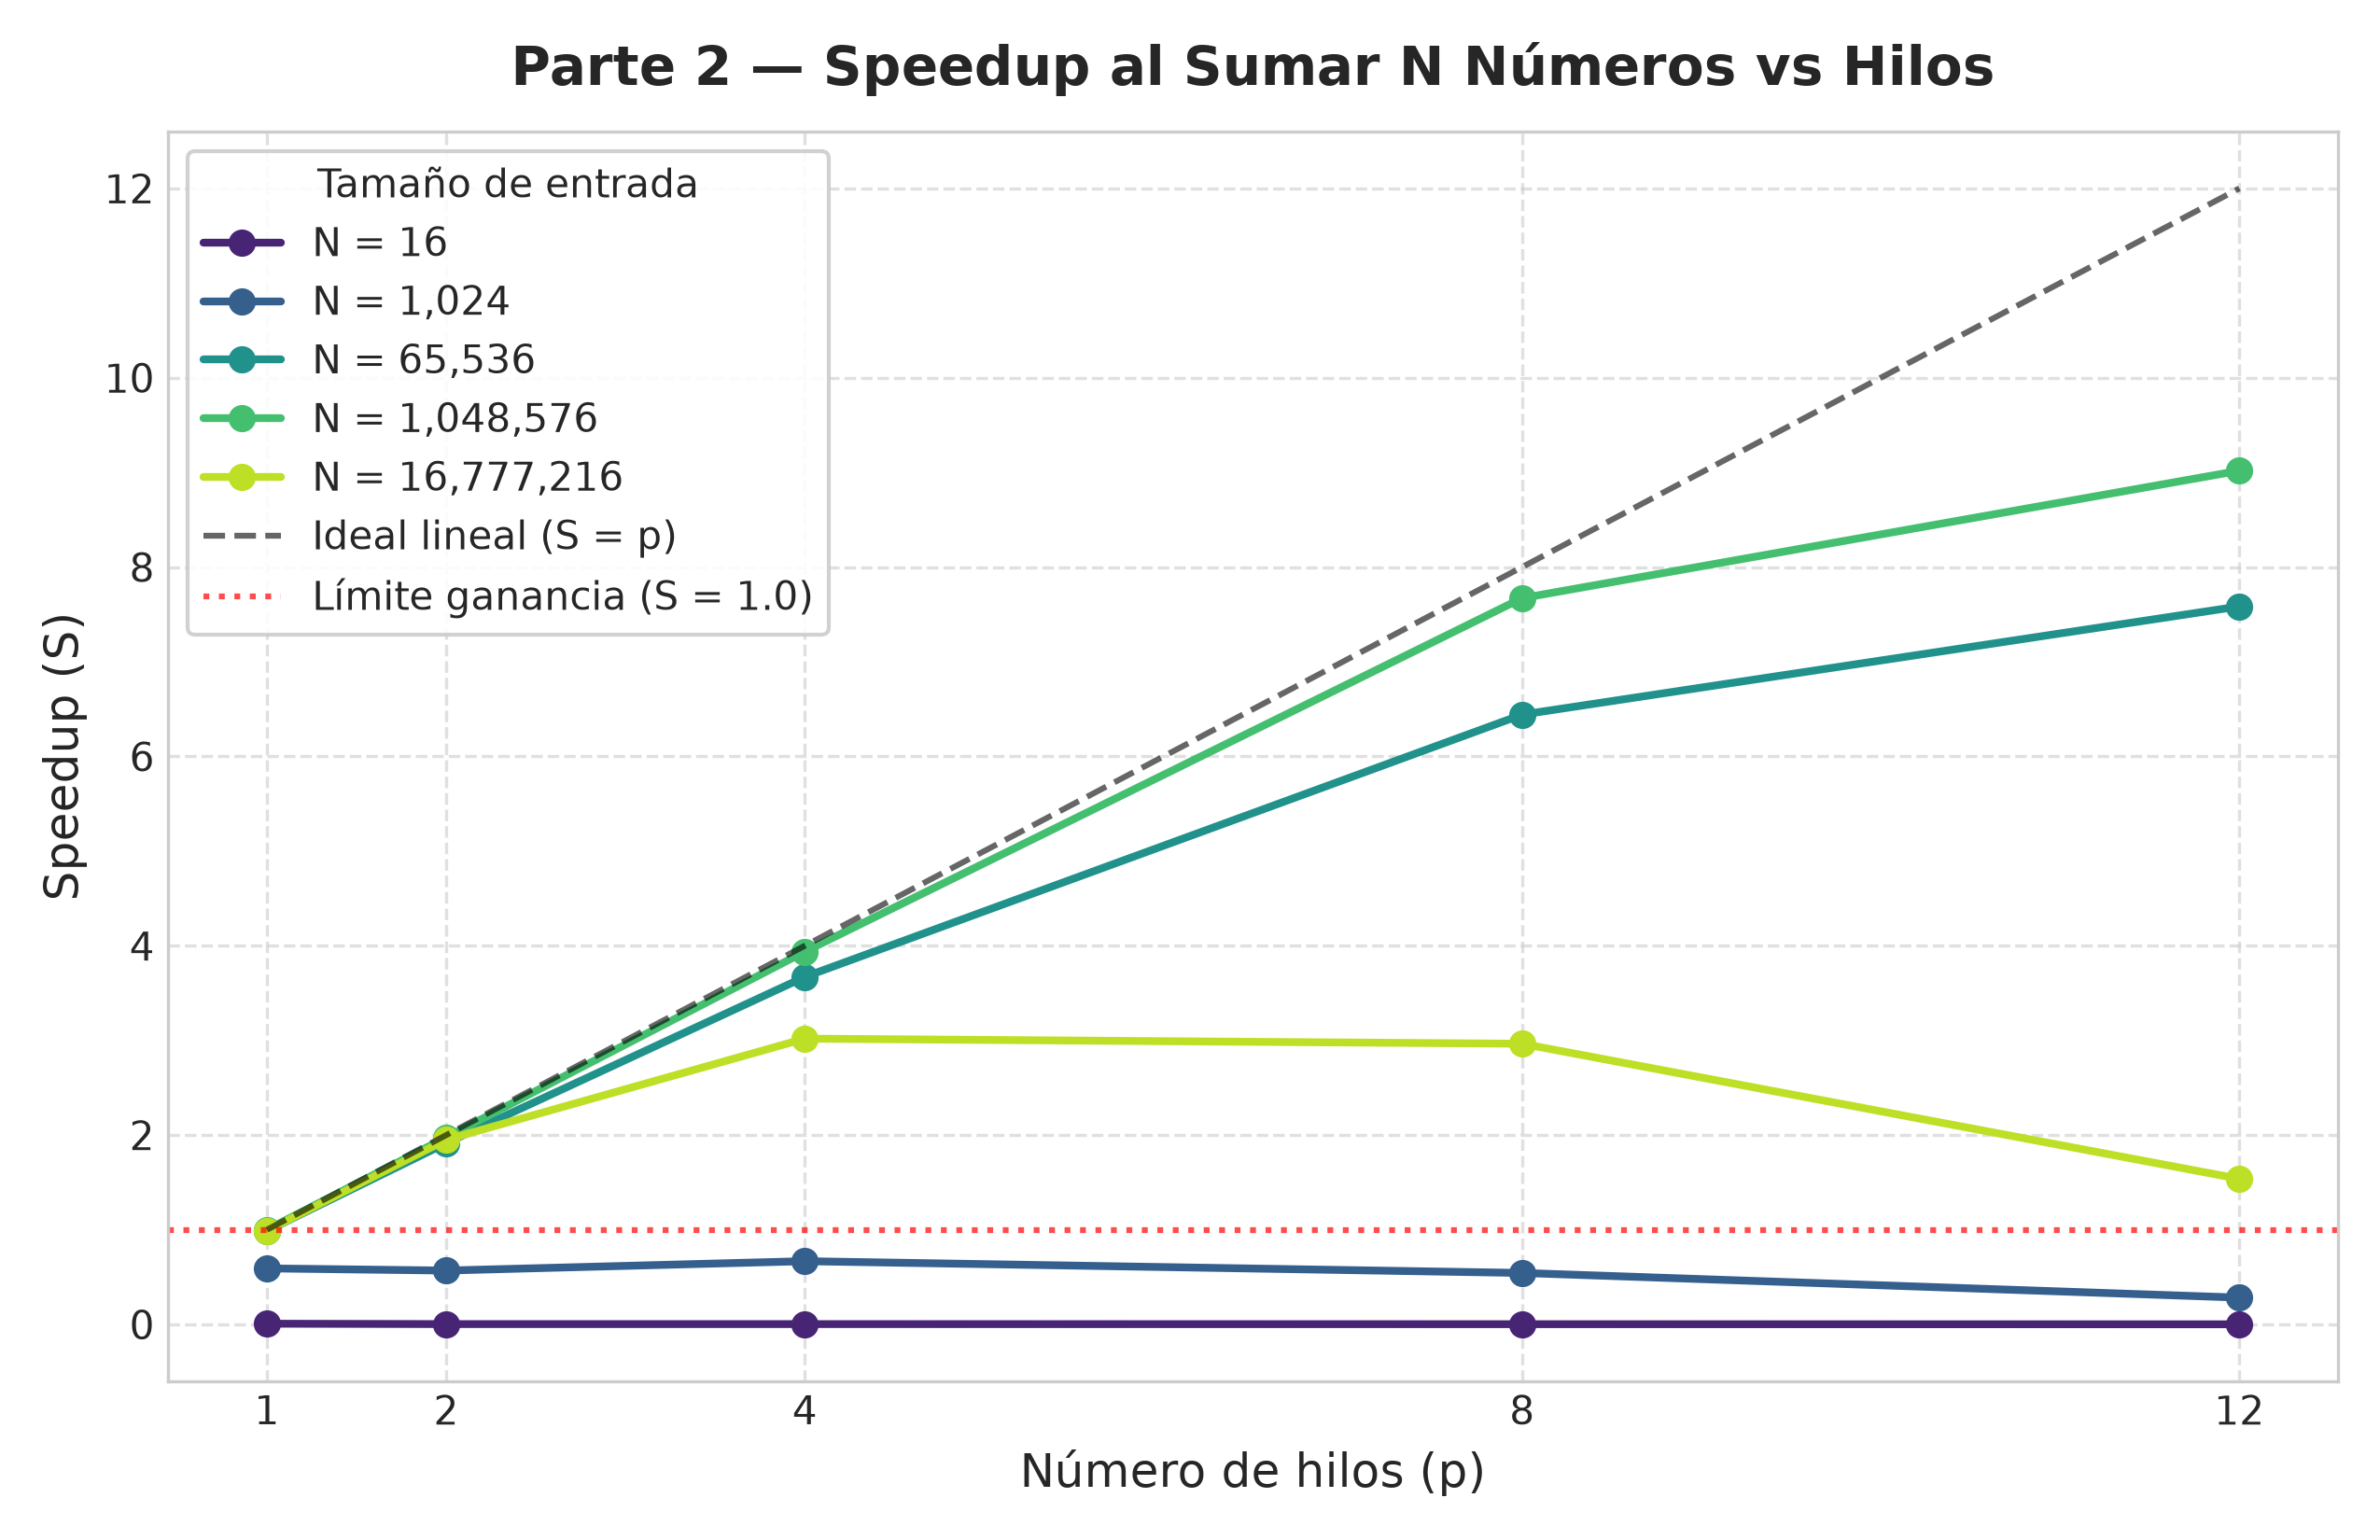
\includegraphics[width=0.88\textwidth]{grafica_suma_speedup.png}
\caption{Gráfica 3 — Speedup vs. hilos para diferentes tamaños de entrada $N$.}
\end{figure}

\begin{figure}[H]
\centering
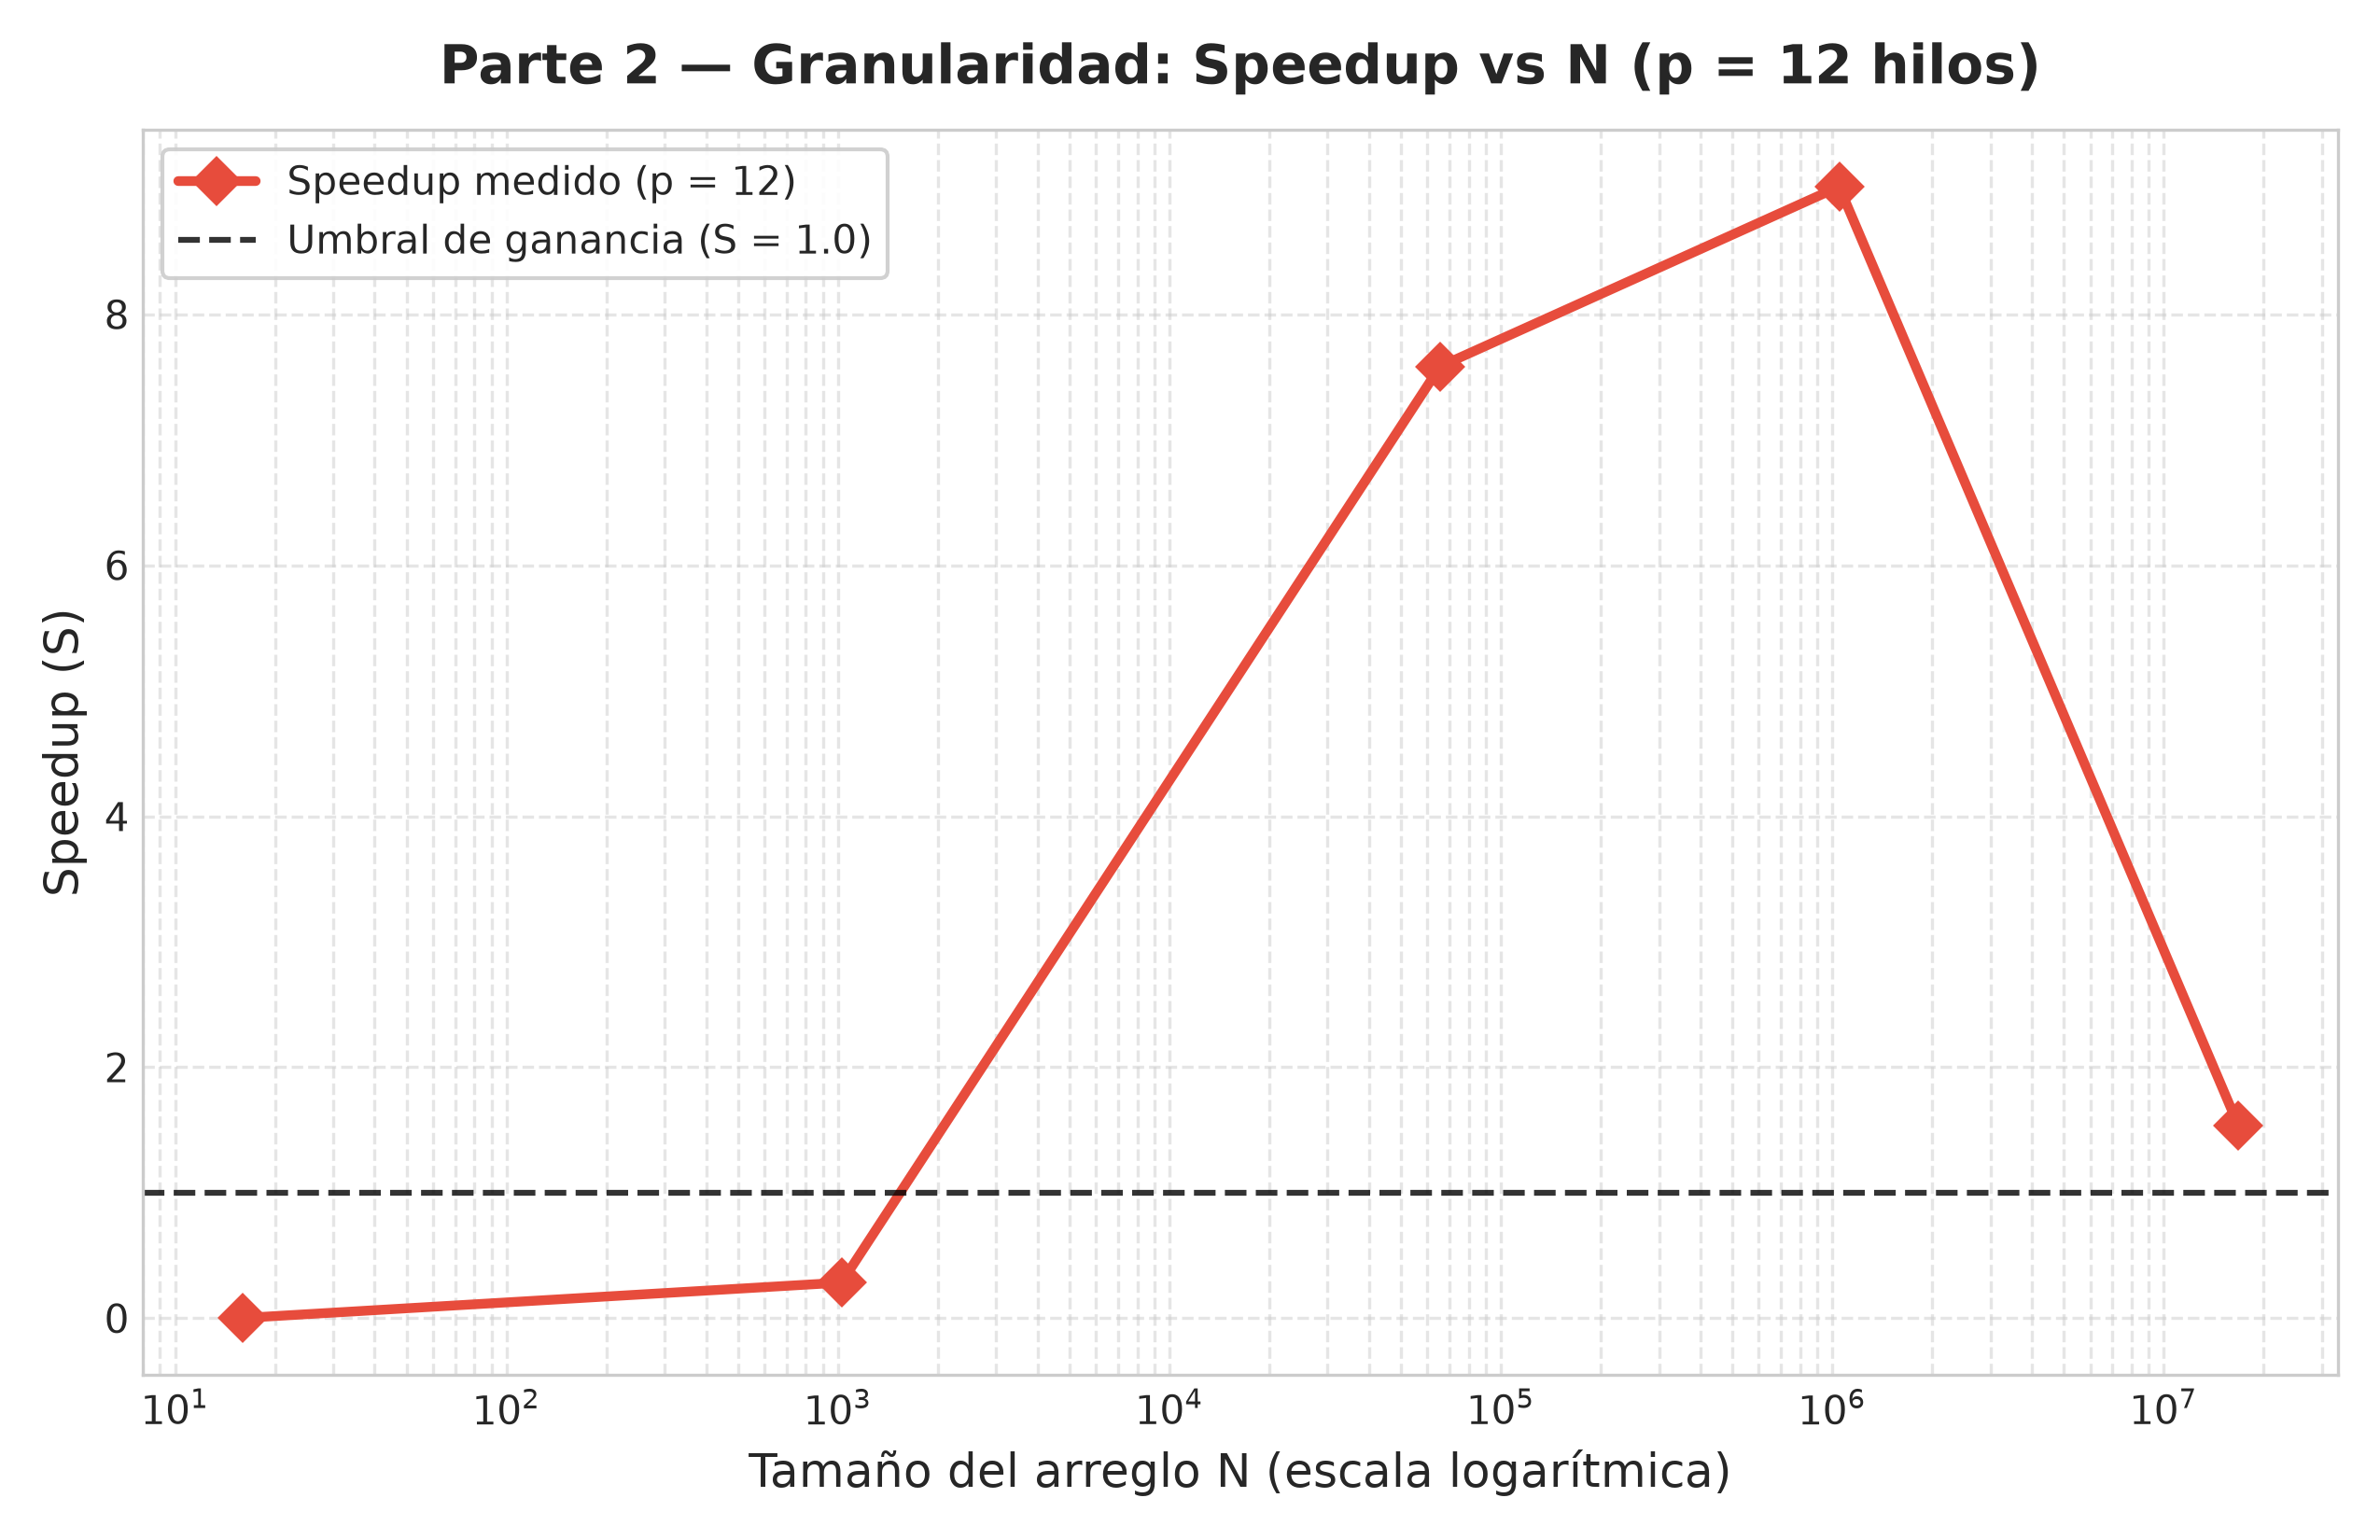
\includegraphics[width=0.88\textwidth]{grafica_suma_granularidad.png}
\caption{Gráfica 4 — Granularidad: Speedup vs. tamaño $N$ en escala logarítmica ($p=12$).}
\end{figure}

\newpage
\subsection{Parte 3: Desbalance de Carga (Gráficas 5 y 6)}
\begin{figure}[H]
\centering
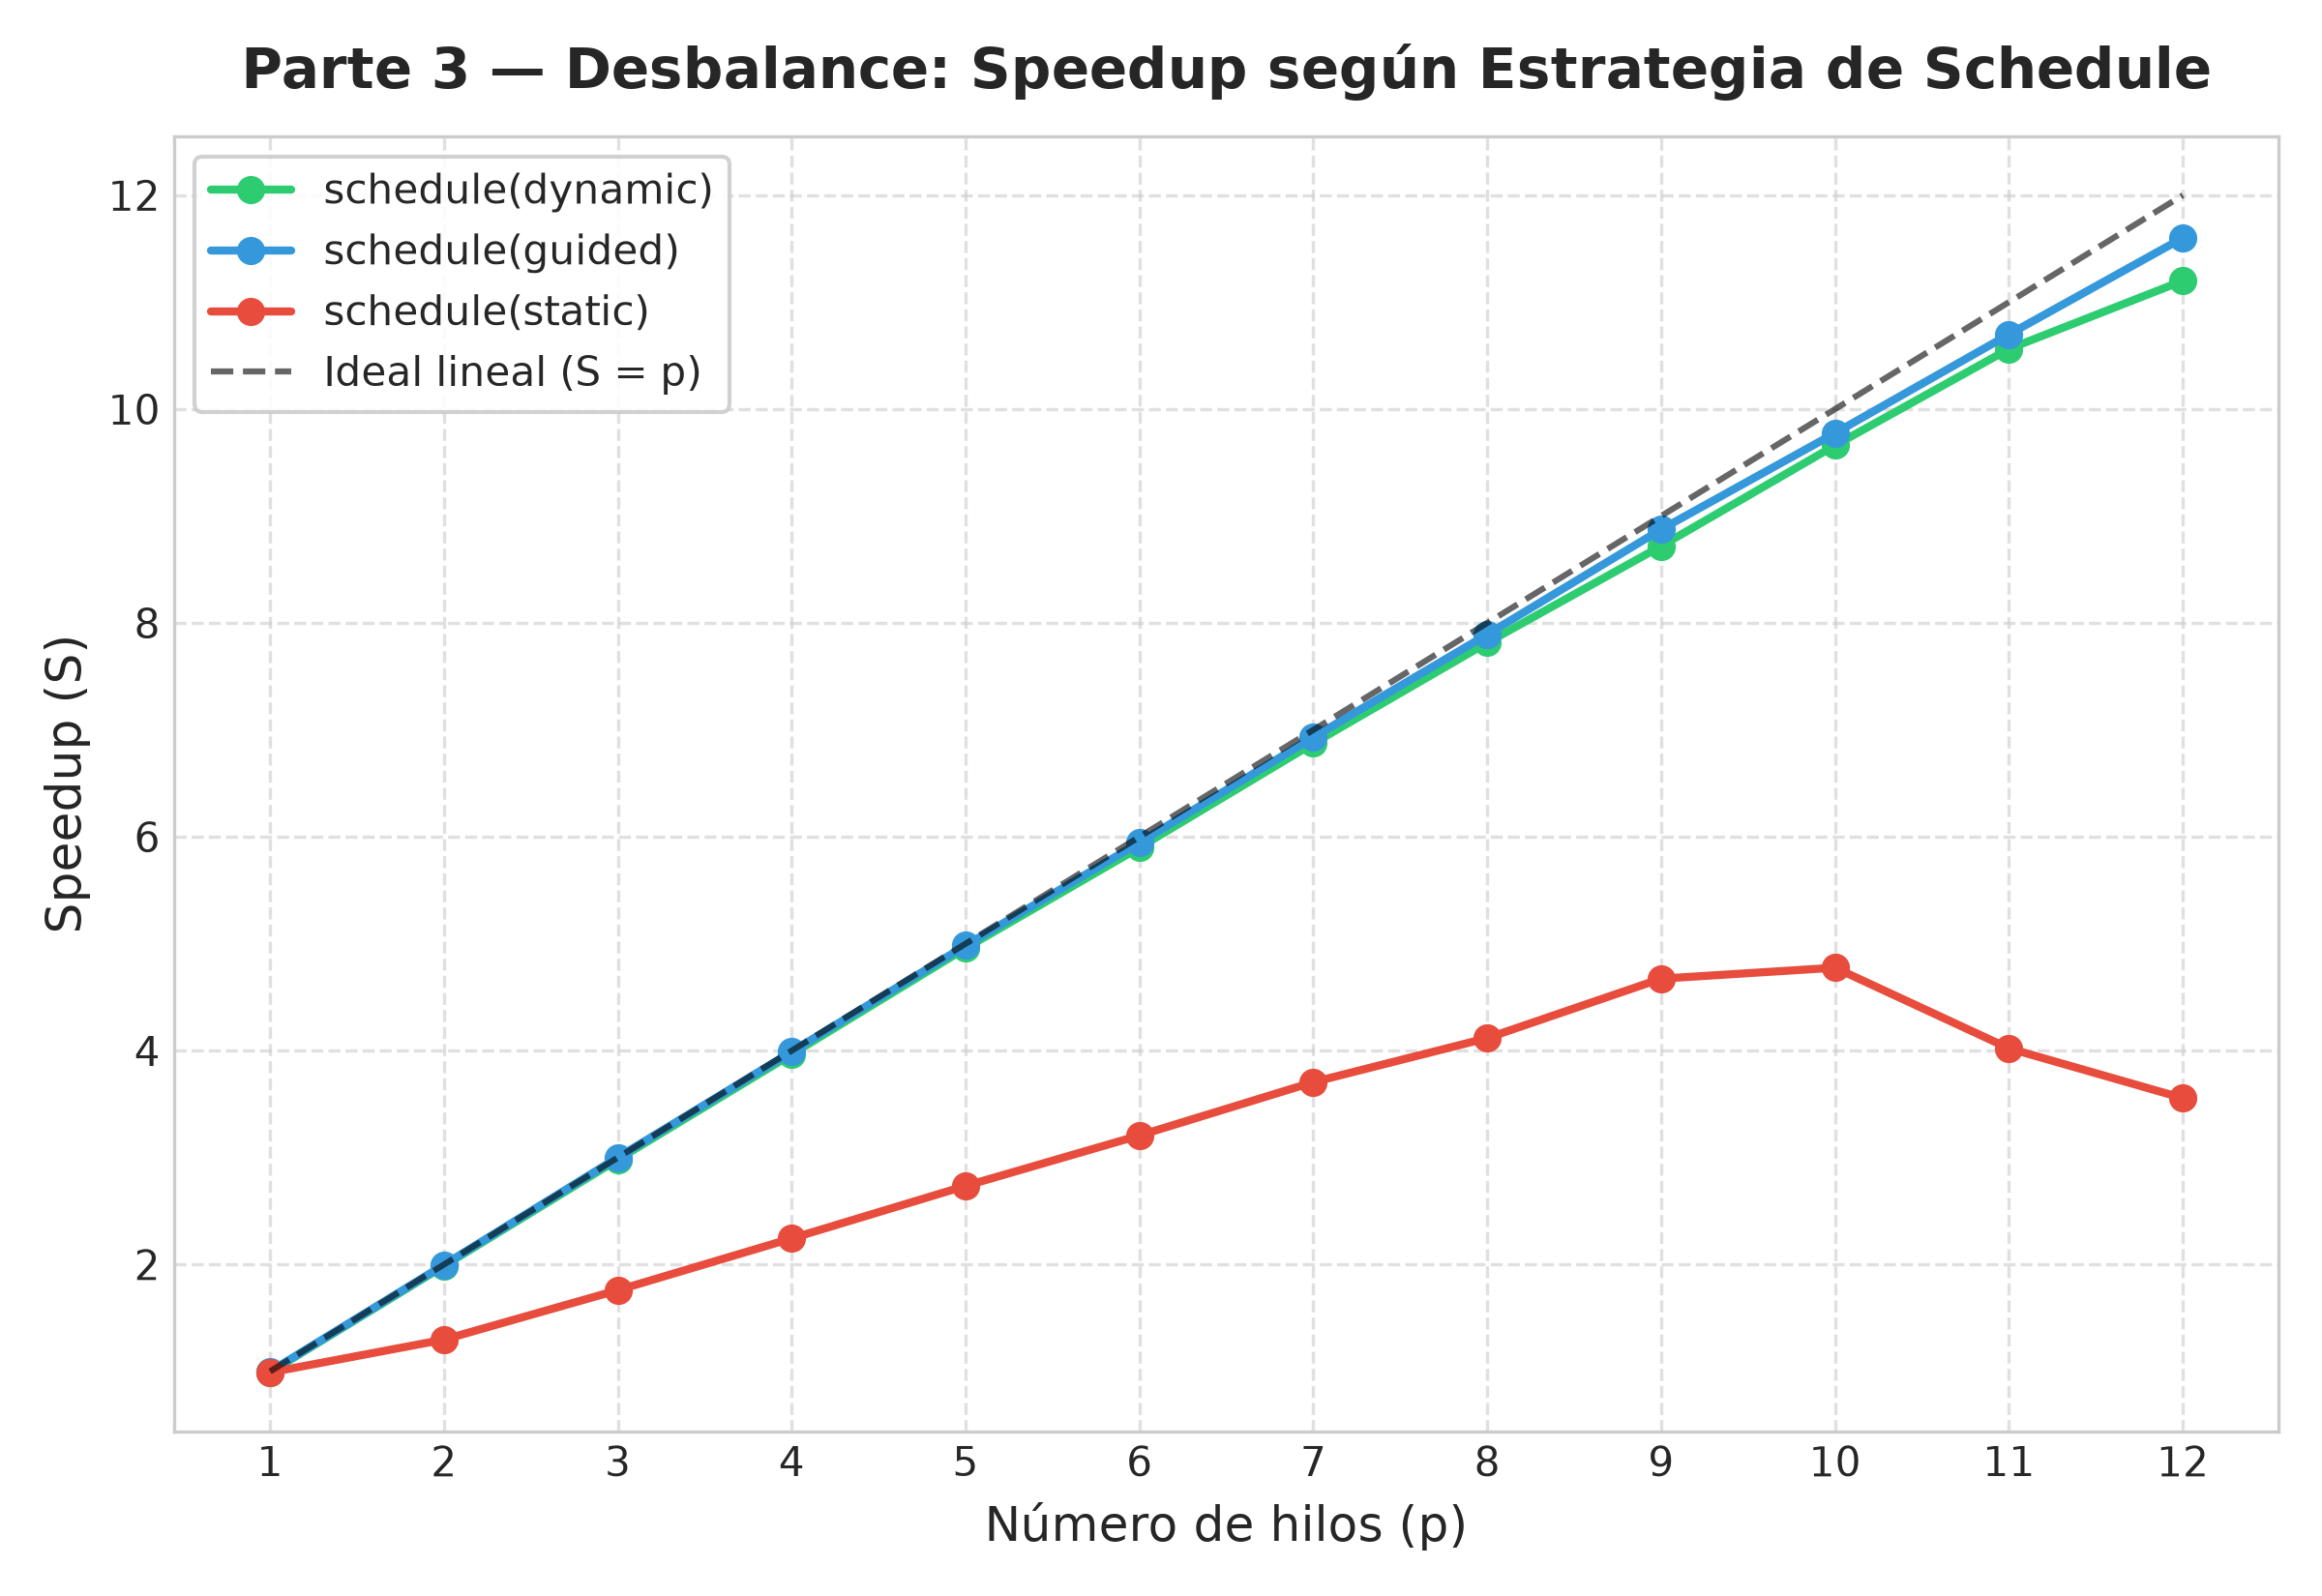
\includegraphics[width=0.88\textwidth]{grafica_desbalance_speedup.png}
\caption{Gráfica 5 — Speedup en presencia de desbalance según schedule (\texttt{static}, \texttt{dynamic}, \texttt{guided}).}
\end{figure}

\begin{figure}[H]
\centering
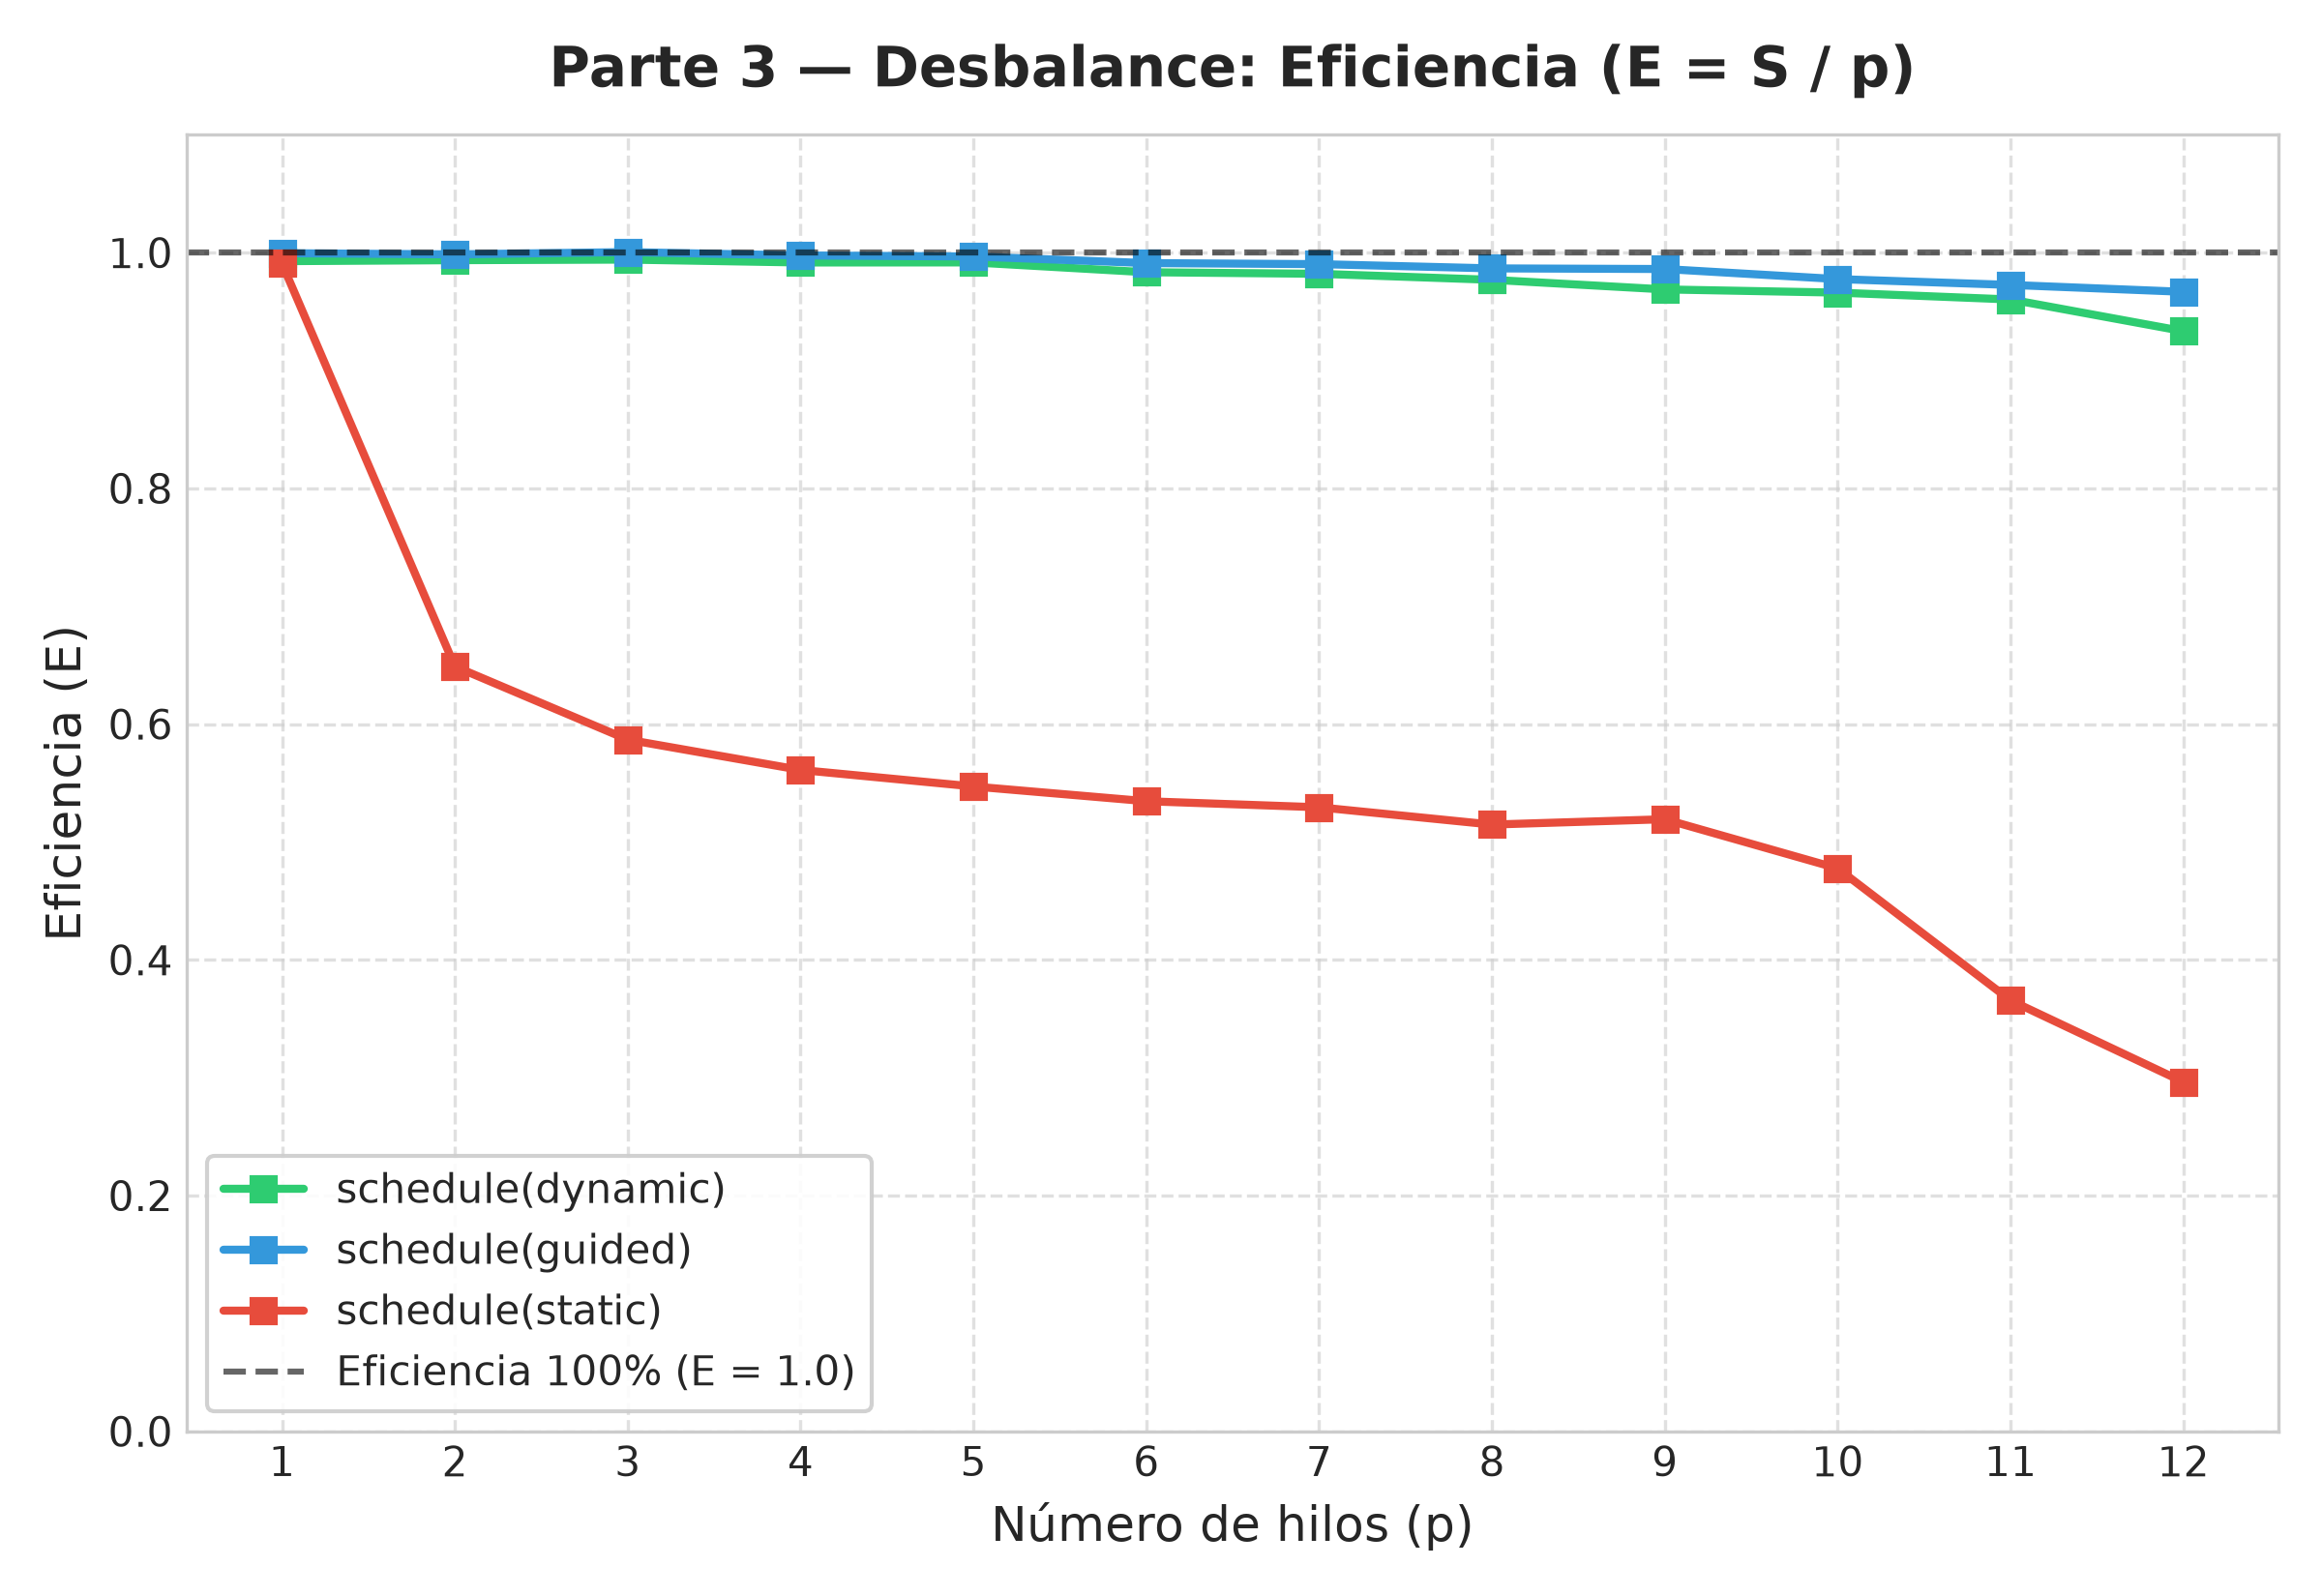
\includegraphics[width=0.88\textwidth]{grafica_desbalance_eficiencia.png}
\caption{Gráfica 6 — Eficiencia en presencia de desbalance según schedule.}
\end{figure}

\newpage
\subsection{Parte 4: Ley de Gustafson (Gráfica 7)}
\begin{figure}[H]
\centering
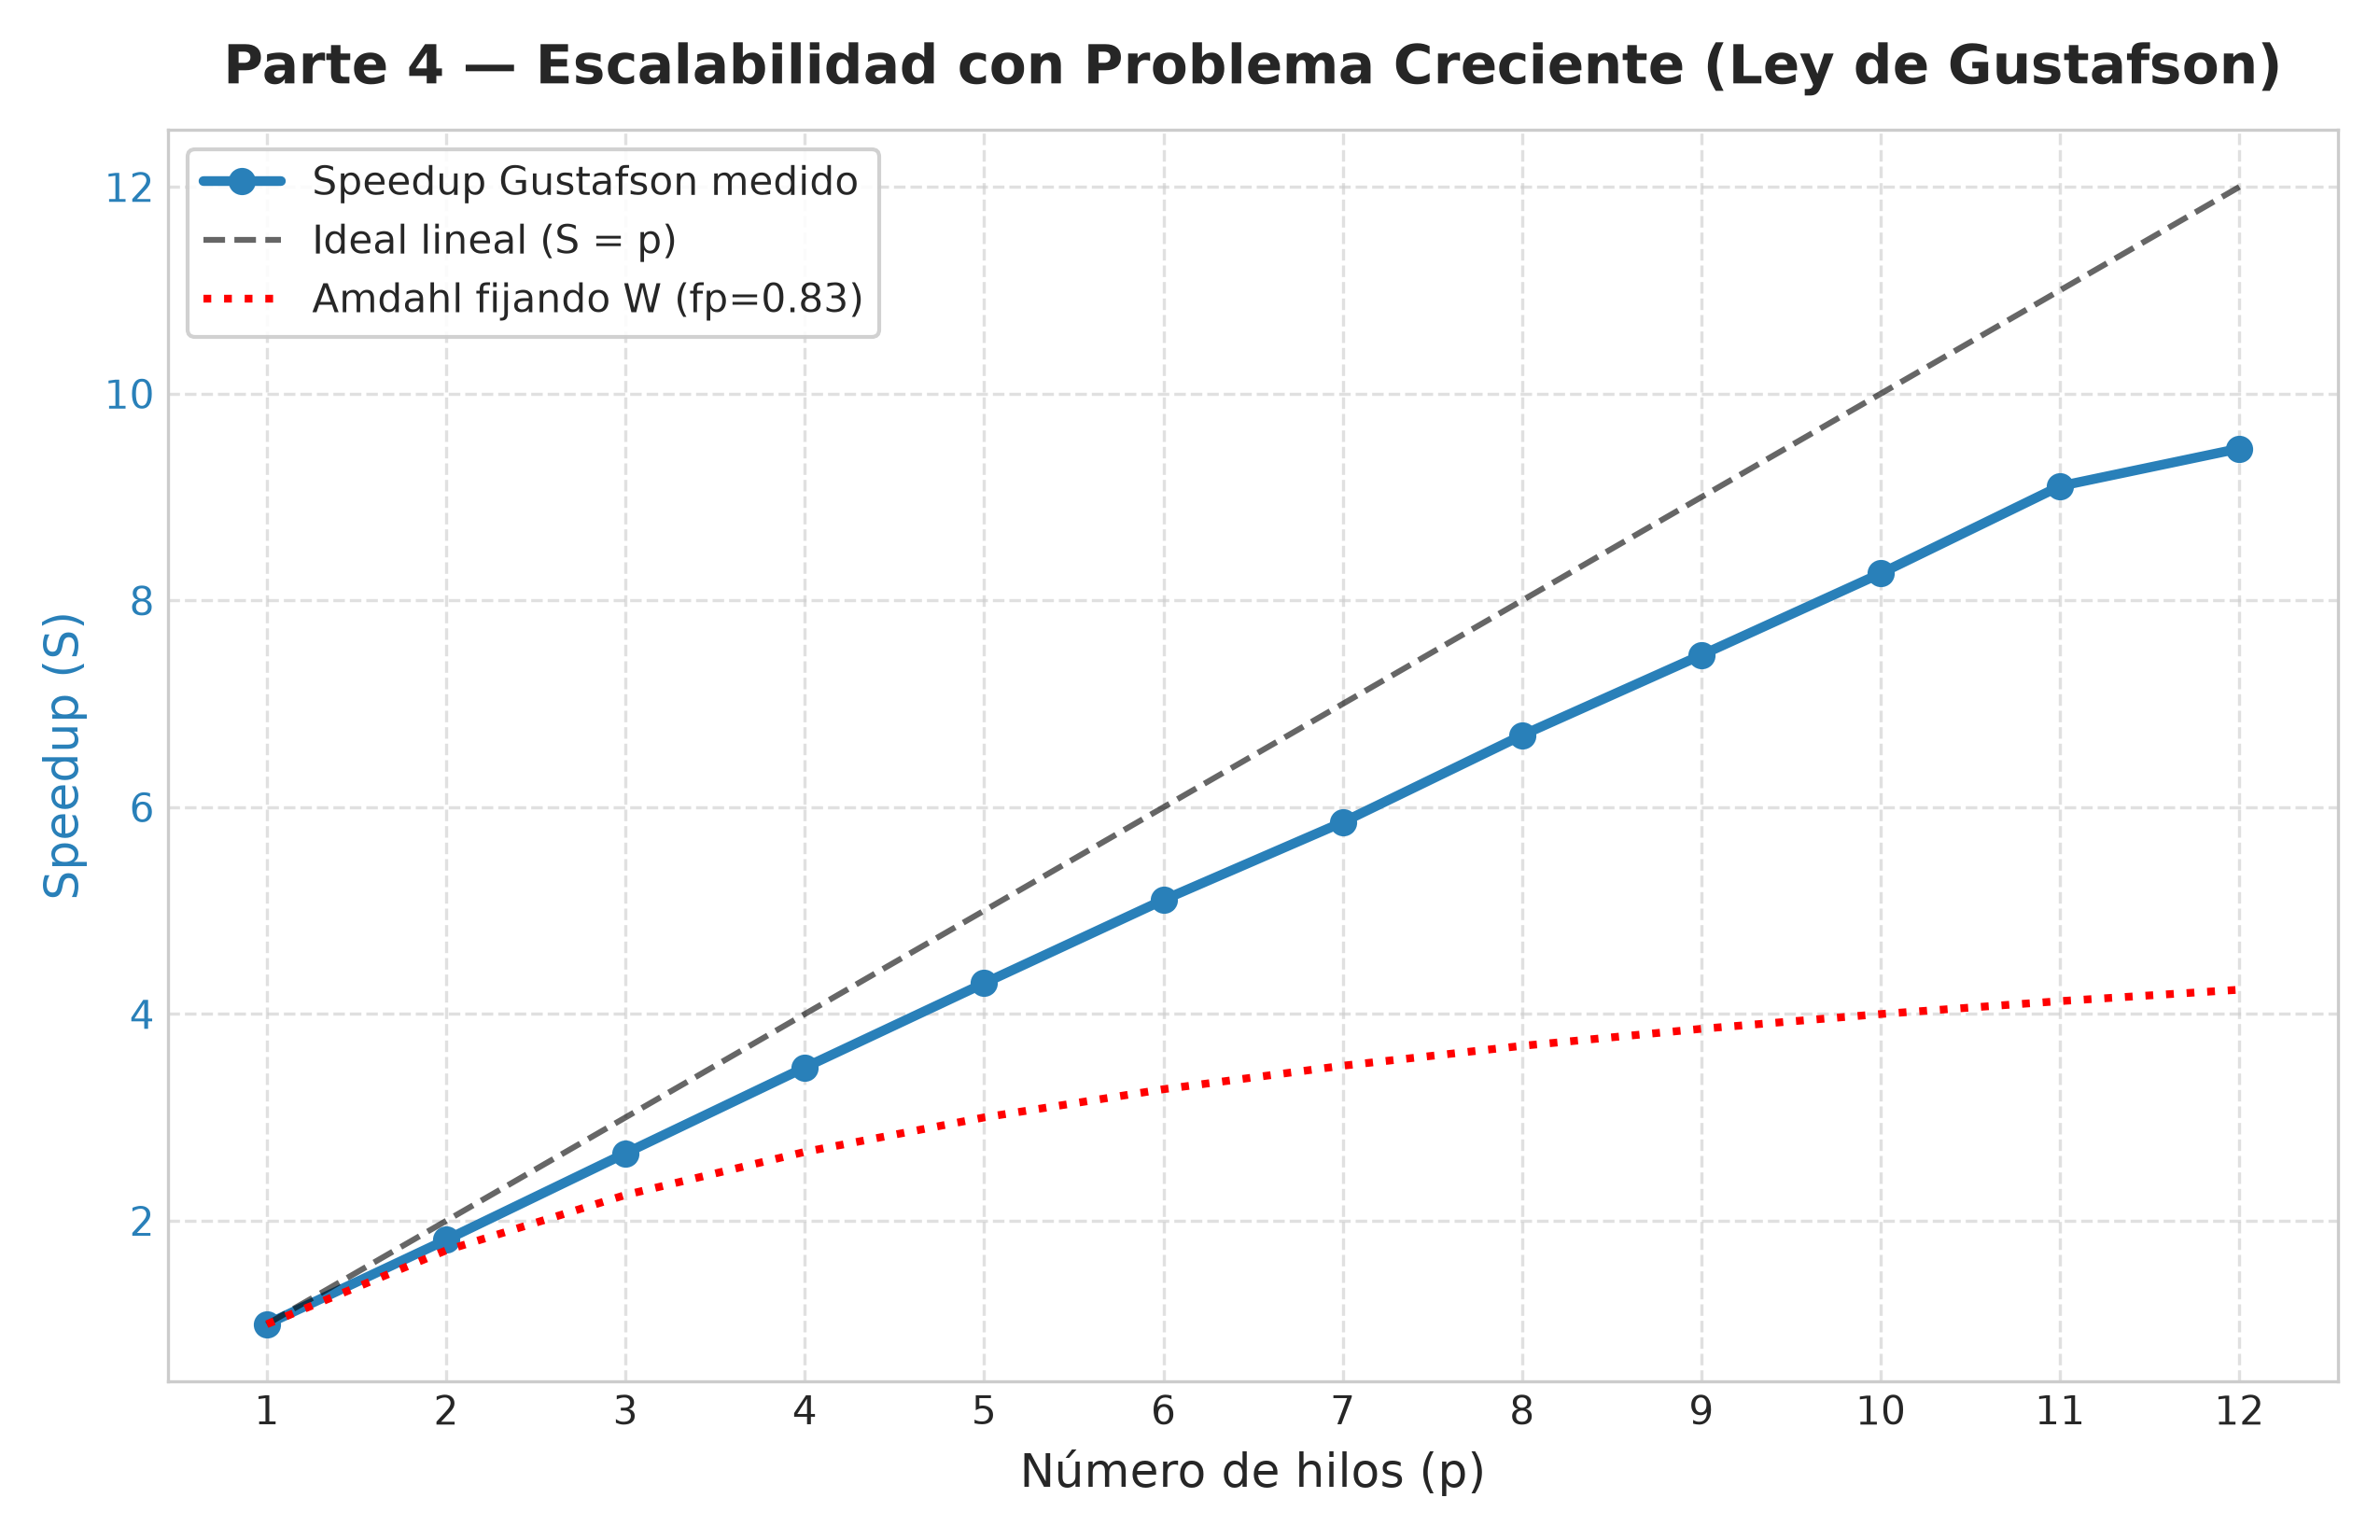
\includegraphics[width=0.88\textwidth]{grafica_gustafson_speedup.png}
\caption{Gráfica 7 — Speedup escalado según la Ley de Gustafson vs. límite fijo de Amdahl.}
\end{figure}

\end{document}
